\documentclass[conference]{IEEEtran}
\IEEEoverridecommandlockouts
% The preceding line is only needed to identify funding in the first footnote. If that is unneeded, please comment it out.
\usepackage{cite}
\usepackage{amsmath,amssymb,amsfonts}
\usepackage{algorithmic}
\usepackage{graphicx}
\usepackage{textcomp}
\usepackage{xcolor}
\def\BibTeX{{\rm B\kern-.05em{\sc i\kern-.025em b}\kern-.08em
    T\kern-.1667em\lower.7ex\hbox{E}\kern-.125emX}}
\begin{document}

\title{Hard disk failure data analysis\\}

\author{\IEEEauthorblockN{Luca Falasca}
\IEEEauthorblockA{\textit{0334722} \\
luca.falasca@students.uniroma2.eu
}
\and
\IEEEauthorblockN{Matteo Conti}
\IEEEauthorblockA{\textit{0323728} \\
matteo.conti97@students.uniroma2.eu
}\\
}


\maketitle

\begin{abstract}
\end{abstract}

\section{Introduzione}
\subsection{Descrizione del problema}
Il problema da affrontare consiste nell'eseguire il batch processing di dati di grandi dimensioni mediante l'uso di una pipeline basata su framework Big Data. Nello specifico, l'obiettivo è analizzare un dataset contenente informazioni relative ai fallimenti dei dischi rigidi per l'esecuzione di 3 query di analisi dei dati e delle prestazioni di esse.

Il dataset fornito è una versione ridotta di quello presentato nel Grand Challenge della conferenza ACM DEBS 2024. Delle numerose colonne presenti nel dataset, ne sono state selezionate cinque per l'esecuzione delle query, in particolare:
\begin{itemize}
    \item \textbf{date}: data della misurazione
    \item \textbf{serial\_number}: identificativo del disco rigido
    \item \textbf{failure}: indica se il disco rigido ha avuto una failure o meno
    \item \textbf{model}: modello del disco rigido
    \item \textbf{vault\_id}: identificativo del gruppo di storage server
    \item \textbf{power\_on\_hours}: ore di accensione del disco rigido
\end{itemize}
\subsection{Obiettivi}
\section{Pipeline}
\subsection{Data Source}
\subsection{Data Ingestion}
\subsection{Data Storage}
\subsection{Data Processing}
Per il processamento dei dati e quindi l'esecuzione delle query è stato utilizzato il framework Spark, in particolare utilizzando la versione per python PySpark.Per queste query è stato utilizzato un cluster composto da uno spark master e quattro spark worker. Per farlo abbiamo utilizzato l'immagine bitami/spark nella versione 3.5.1. Per l'orchestrazione del cluster abbiamo utilizzato docker compose.
Il dataset parzialemente filtrato è stato caricato dall'hdfs e i risultati delle query sono stati salvati in mongodb utilizzando il connettore spark-mongodb.
Le query sono state eseguite sia a partire da file in formato CSV che in formato Parquet per valutare le differenze di prestazioni tra un formato basato su colonne e uno basato su righe.
\subsubsection{Query 1}
\subsubsection{Query 2}
\subsubsection{Query 3}
\subsection{Analytical Data Storage}
I risultati delle query sono stati memorizzati in un database MongoDB (Fig. \ref{fig:mongo}).
Per organizzare i dati, abbiamo creato una collezione per ciascuna query, dove ogni documento rappresenta una riga dei risultati ottenuti dalla query stessa. Inoltre, abbiamo un'altra collezione che contiene i risultati, includendo il timestamp dell'esperimento, la query specifica e il formato con cui è stata eseguita, oltre al tempo impiegato per l'esecuzione.

\begin{figure}[htbp]
    \centerline{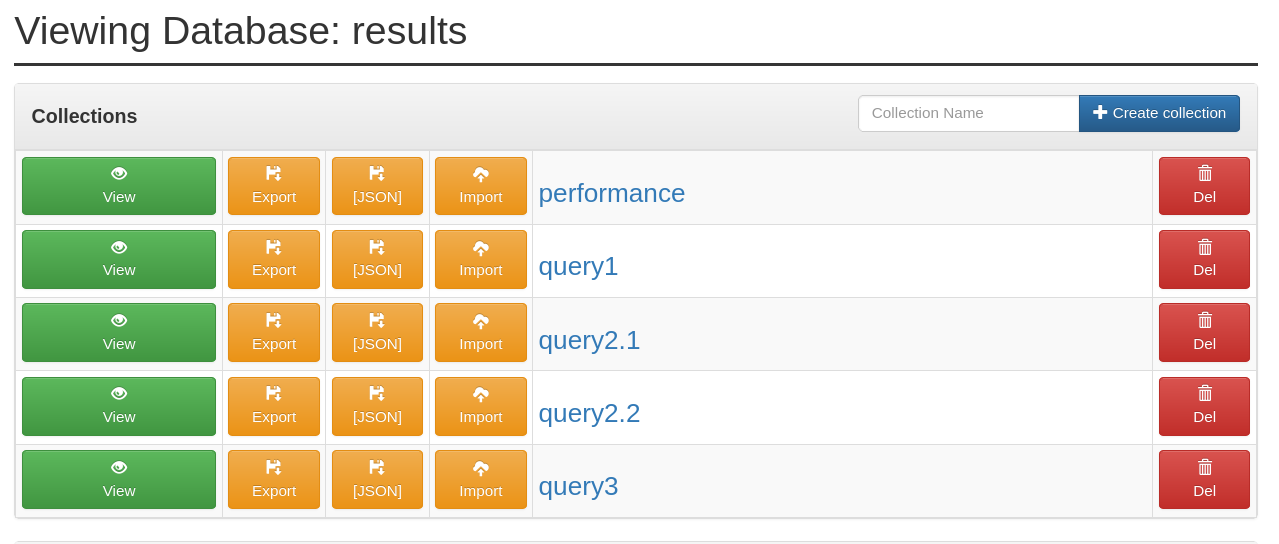
\includegraphics[width=0.5\textwidth]{res/mongo.png}}
    \caption{Schema del database MongoDB.}
    \label{fig:mongo}
\end{figure}
\subsection{Visualization}
\subsection{Analisi delle prestazioni}
\section*{References}

Please number citations consecutively within brackets \cite{b1}. The 
sentence punctuation follows the bracket \cite{b2}. Refer simply to the reference 
number, as in \cite{b3}---do not use ``Ref. \cite{b3}'' or ``reference \cite{b3}'' except at 
the beginning of a sentence: ``Reference \cite{b3} was the first $\ldots$''

Number footnotes separately in superscripts. Place the actual footnote at 
the bottom of the column in which it was cited. Do not put footnotes in the 
abstract or reference list. Use letters for table footnotes.

Unless there are six authors or more give all authors' names; do not use 
``et al.''. Papers that have not been published, even if they have been 
submitted for publication, should be cited as ``unpublished'' \cite{b4}. Papers 
that have been accepted for publication should be cited as ``in press'' \cite{b5}. 
Capitalize only the first word in a paper title, except for proper nouns and 
element symbols.

For papers published in translation journals, please give the English 
citation first, followed by the original foreign-language citation \cite{b6}.

\begin{thebibliography}{00}
\bibitem{b1} G. Eason, B. Noble, and I. N. Sneddon, ``On certain integrals of Lipschitz-Hankel type involving products of Bessel functions,'' Phil. Trans. Roy. Soc. London, vol. A247, pp. 529--551, April 1955.
\bibitem{b2} J. Clerk Maxwell, A Treatise on Electricity and Magnetism, 3rd ed., vol. 2. Oxford: Clarendon, 1892, pp.68--73.
\bibitem{b3} I. S. Jacobs and C. P. Bean, ``Fine particles, thin films and exchange anisotropy,'' in Magnetism, vol. III, G. T. Rado and H. Suhl, Eds. New York: Academic, 1963, pp. 271--350.
\bibitem{b4} K. Elissa, ``Title of paper if known,'' unpublished.
\bibitem{b5} R. Nicole, ``Title of paper with only first word capitalized,'' J. Name Stand. Abbrev., in press.
\bibitem{b6} Y. Yorozu, M. Hirano, K. Oka, and Y. Tagawa, ``Electron spectroscopy studies on magneto-optical media and plastic substrate interface,'' IEEE Transl. J. Magn. Japan, vol. 2, pp. 740--741, August 1987 [Digests 9th Annual Conf. Magnetics Japan, p. 301, 1982].
\bibitem{b7} M. Young, The Technical Writer's Handbook. Mill Valley, CA: University Science, 1989.
\end{thebibliography}
\vspace{12pt}


\end{document}